\documentclass[10pt, a4paper, twocolumn]{article}

\usepackage[english]{babel}
\usepackage{float}
\usepackage{graphicx}
\usepackage[margin=0.5in]{geometry}
\usepackage{hyperref}
\usepackage{listings}

\title{{\Large \textbf{EN2550 Assignment 04\\
{\LARGE Classification of CIFAR-10 image dataset}}}}
\author{{\large 180616T P.M.P.H.Somarathne}}
\date{\tiny}

\begin{document}

\maketitle
Full code is available at \url{https://git.io/JYgRe}\\
Used $10\%$ of training set as validation.\\
Training data size : (45000, 3072)\\
Training label size : (45000, 10)\\
Validation data size: (5000, 3072) \\
Validation label size: (5000, 10)\\
Test data size : (10000, 3072)\\
Test label size : (10000, 10)\\
No of classes : 10\\
The models were trained on Google Colab and Kaggle platforms.

\section{Linear classifier}
\subsection{Model}
Linear model is based on $f(x) = Wx + b$, where $W$ is the weights matrix of shape $(3072,10)$ and $b$ is the bias vector of shape $(1,10)$. Started training with initial learning rate of $0.017$ with a decay factor of $0.1\%$ and L2 regularization parameter of $1 \times 10^{-6}$. The loss function is the mean sum of squared errors with L2 regularization. The governing equations of the model are as follows.\\
Forward propagation: {\small \[f(x) = Wx + b\]}
Loss function: {\small \[J = \frac{1}{m}\sum_{l=0}^{m}\sum_{k=0}^{9}(y_{pred,l,k}-y_{l,k})^{2} + \lambda\sum_{(i,j) = (0,0)}^{(3071,9)} W_{i,j}\]} where $m$ is the number of samples, $\lambda$ is the regularization parameter, $l$ iterates over the samples, $k$ iterates over the classes and $W_{i,j}$ is the $i^{th},j^{th}$ element of weights matrix.\\
Back-propagation:{\small 
\[\frac{\partial J}{\partial W} = \frac{2}{m}x'(y_{pred}-y)\]
\[\frac{\partial J}{\partial b} = \frac{2}{m}\sum_{l=0}^{m}(y_{pred,l}-y_{l})\]}
Gradient-descent:{\small 
\[W = W - \alpha \frac{\partial J}{\partial W} - \alpha \lambda W\]
\[b = b - \alpha \frac{\partial J}{\partial b}\]} where $\alpha$ is the learning rate for the given iteration.\\
Accuracy calculation(top-one accuracy):{\small 
\[Accuracy = \frac{No.\ of\ correct\ class\ predictions}{Total\ no.\ of\ predictions}\times 100\%\]}

\subsection{Results}
\begin{figure*}
  \centering
	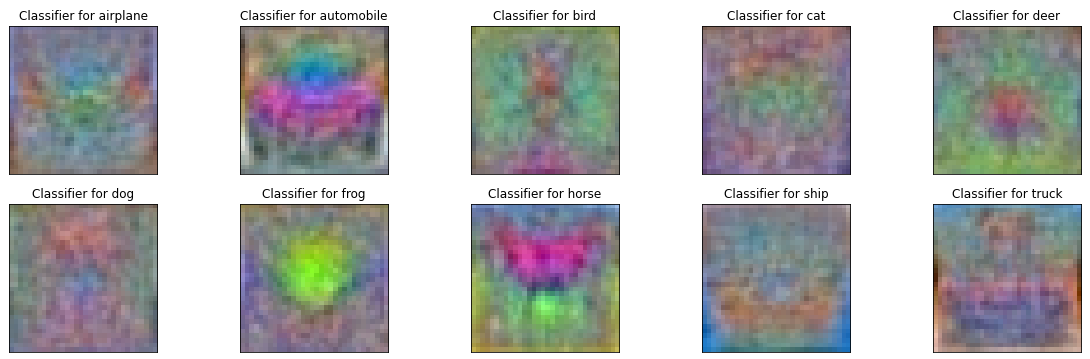
\includegraphics[width=.9\textwidth]{./images/linearClasses.png}
	\caption{\textit{The weight matrices interpreted as images. The images resemble the classes they represent(specially in the horse image). Cat and dog classes have low resemblance; the reason could be that cat and dog images are very common and they vary greatly between the breeds(of dogs), the posture of the animal and the background(in a house vs. outside).}}
	\label{fig:linClas}
\end{figure*}
\begin{figure}
	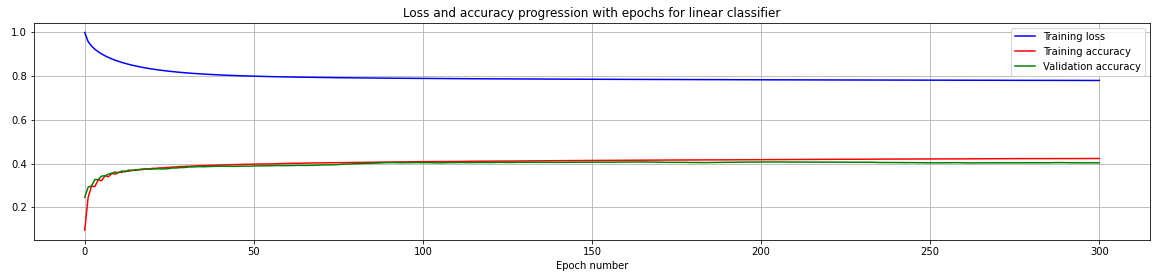
\includegraphics[width=.49\textwidth]{./images/linearLoss.png}
	\caption{\textit{Progression of training loss, training accuracy and validation accuracy of linear classifier with each epoch}}
	\label{fig:linLoss}	
\end{figure}
Training elapsed for 7 minutes. The trained weight matrix is depicted as images for each class in figure \ref{fig:linClas}. These images slightly resemble the class they represent; specially the object colors, object shape(loosely) and background colors are there.The progression of training loss, training accuracy and validation accuracy are shown in figure \ref{fig:linLoss}. The final training accuracy is $42.39\%$ and validation accuracy is $40.4\%$. The accuracy for the test set is $40.6\%$. The differences between training accuracy and test/validation accuracy are small so we can conclude that the model has not over-fitted the data. However, it is clear that the values have changed very slightly after $50^{th}$ epoch. The reason could be that the model is too simple(high bias case) to fit the data. Furthermore, adding shuffling of dataset in each epoch has reduced the gap between the training accuracy and validation/test accuracy, making the model more biased, but in-turn helping the model to generalize well.

\section{2-layer neural network classifier}
\subsection{Model}
The implemented neural network has 200 hidden nodes with sigmoid activation and 10 output nodes without activation. The model was trained with an initial learning rate of $0.015$ with $0.01\%$ decay and L2 regularization parameter of $1 \times 10^{-6}$. The loss function was mean sum of squared errors with L2 regularization. One issue faced when implementing this model was that the gradients were too small and they failed to propagate back through the layers with enough accuracy. In order to fix this, I have changed the range of input from normalized([0.0 - 1.0]) range used earlier, to 0.0-100.0 range. This has increased the gradients to a sufficient level to carryout back-propagation properly. The governing equations of this model are as follows.\\
Forward propagation: {\small
\[a_{1} = sigmoid(W_{1} x + b_{1})\]
\[y_{pred} = W_{2} a_{1} + b_{2}\]}
Loss function: {\small \[J = \frac{1}{m}\sum_{l=0}^{m}\sum_{k=0}^{9}(y_{pred,l,k}-y_{l,k})^{2} + \lambda\sum_{(i,j) = (0,0)}^{(3071,199)} W_{1}(i,j)\]
\[ + \lambda\sum_{(i,j) = (0,0)}^{(199,9)} W_{2}(i,j)\]} where $m$ is the number of samples, $\lambda$ is the regularization parameter, $l$ iterates over the samples, $k$ iterates over the classes and $W_{L}(i,j)$ is the $i^{th},j^{th}$ element of weights matrix of layer $L$.\\
Back-propagation:{\small 
\[\frac{\partial J}{\partial W_{1}} = \frac{2}{m}a_{1}'(y_{pred}-y)\]
\[\frac{\partial J}{\partial b_{1}} = \frac{2}{m}\sum_{l=0}^{m}(y_{pred,l}-y_{l})\]
\[\frac{\partial J}{\partial W_{2}} = \frac{2}{m} x' a_{1} (1-a_{1})(y_{pred}-y)W_{2}\]
\[\frac{\partial J}{\partial b_{2}} = \frac{2}{m}\sum_{l=0}^{m} a_{1} (1-a_{1}) (y_{pred,l}-y_{l})W_{2}\]}
Gradient-descent:{\small 
\[W_{1} = W_{1} - \alpha \frac{\partial J}{\partial W_{1}} - \alpha \lambda W_{1}\]
\[b_{1} = b-{1} - \alpha \frac{\partial J}{\partial b_{1}}\]
\[W_{2} = W_{2} - \alpha \frac{\partial J}{\partial W_{2}} - \alpha \lambda W_{2}\]
\[b_{2} = b_{1} - \alpha \frac{\partial J}{\partial b_{2}}\]} where $\alpha$ is the learning rate for the given iteration.
\subsection{Results}
\begin{figure}
  \centering
	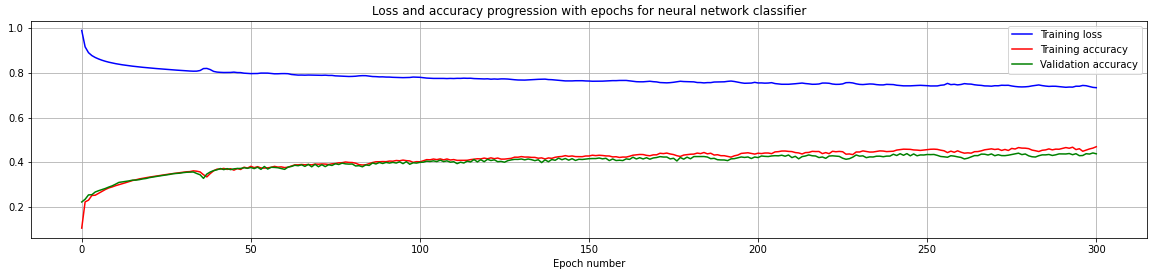
\includegraphics[width=.49\textwidth]{./images/nn1Loss.png}
	\caption{\textit{Progression of training loss, training accuracy and validation accuracy of neural network classifier with each epoch}}
	\label{fig:nn1Loss}
\end{figure}
Neural network took 25 minutes to train. The progression of metrics are shown in figure \ref{fig:nn1Loss}. The final training accuracy is $47.0\%$ and final validation accuracy is $43.84\%$. The model showed $43.53\%$ accuracy on the test set. The progression of training accuracy and validation accuracy shows that the model has not over-fitted to training data. This model has higher accuracy than the linear model; but still the accuracy is less than $50\%$. It could be slightly increased by tuning the parameters more. The accuracy might be greatly improved by applying an activation function(like softmax) for the output layer and adding another hidden layer.

\section{2-layer neural network with stochastic gradient descent (SGD)}
\subsection{Model}
Instead of using all 45000 of the samples to do one step of gradient descent, this method does it for smaller groups of samples, namely mini-batches. With the shuffling of training data in each epoch, it maintains a uniform distribution within the training data and then splits the data into 90 mini-batches of size 500 each. It runs the steps of part 2 on a 500 group and proceed to next group. This way, when it goes through the dataset once, the gradient would've descended 90 times and would surpass the gradient descent approach in less number of epochs.\\
The model is run with a learning rate of $0.001$ with decay of $5\%$ and L2 regularization parameter of $1 \times 10^{-3}$. The input range adjustment was added to this model, similar to model in part 2.
\subsection{Results}
\begin{figure}
  \centering
	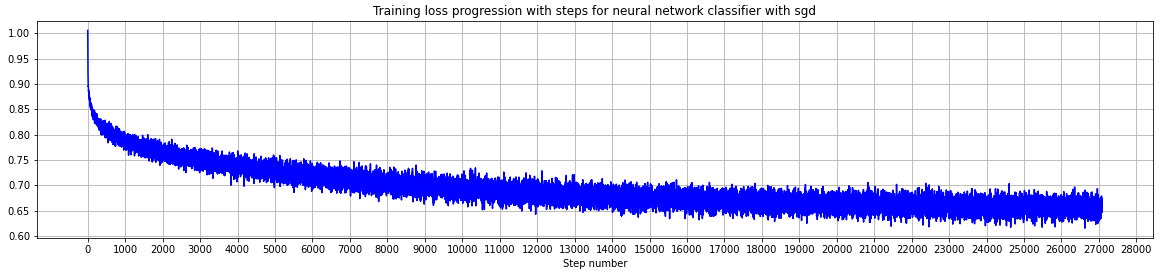
\includegraphics[width=.49\textwidth]{./images/nn2Loss.png}
	\caption{\textit{Progression of training loss of neural network classifier with SGD in each step}}
	\label{fig:nn2Loss}
\end{figure}
\begin{figure}
  \centering
	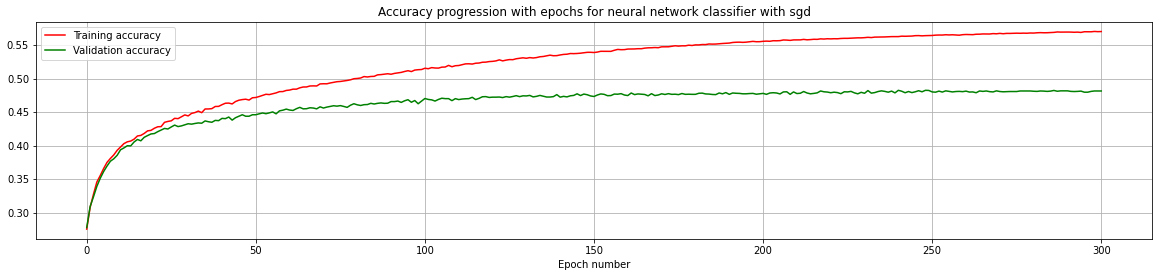
\includegraphics[width=.49\textwidth]{./images/nn2Acc.png}
	\caption{\textit{Progression of accuracy of neural network classifier with SGD in each epoch}}
	\label{fig:nn2Acc}
\end{figure}
SGD took 41 minutes to train but reached a higher accuracy. Figure \ref{fig:nn2Acc} shows the progression of training accuracy and validation accuracy. After around $60^{th}$ epoch, the training accuracy tends to increase faster than validation accuracy and create a considerable gap between those two. This can be taken as evidence of model over-fitting to the training data. More tuning of parameters may reduce this gap slightly. The final training accuracy is $57.03\%$, final validation accuracy is $48.18\%$ and the test accuracy is $47.27\%$. The most interesting part of the results of this model is the progression of training loss across each step($1/100^{th}$ of an epoch), shown in figure \ref{fig:nn2Loss}. The line has lot of noise due to small groups having slightly different features/ distributions and different no of images from a given class. However, the loss has an overall decreasing trend.\\
Let's compare this with the loss and accuracy from previous neural network implementation(refer figure \ref{fig:nn1v2}). The model with SGD surpasses the model in part 2 after $5$ minutes which was at $40^{th}$ epoch. That means it has achieved the previous accuracy in $1/5^{th}$ of the time. Addition of SGD has greatly reduced training time. But, when it reaches the final epochs, over-fitting becomes a major issue. Stopping the model when the required accuracy is reached, would be the reasonable option to get high accuracy model in less amount of time. I ran the model for 300 epochs without stopping to observe its behavior.

\section{CNN implementation with Keras}
\subsection{Model}
The model has three convolution layer followed by maxpool layer pairs, a flatten layer and two fully connected layers. Maxpool layers and flatten layer have no learnable parameters. The number of parameters in other layers are shown in table \ref{table: tab1}. The number of total learnable parameters of the network is $122,570$. The activation function of each layer are shown in brackets of column one of table \ref{table: tab1}.
\begin{table}
\centering
\begin{tabular}{|l|r c|}
\hline
Layer &Parameters &\\
\hline
C32(sigmoid) & $ [3 \times (3 \times 3) + 1] \times 32 =$ &896\\
C64\_1(sigmoid) & $ [32 \times (3 \times 3) + 1] \times 64 =$ &18496\\
C64\_2(sigmoid) & $ [64 \times (3 \times 3) + 1] \times 64 =$ &36928\\
F64(sigmoid) & $ [64 \times (4 \times 4) + 1] \times 64 =$ &65600\\
F10(softmax) & $ [64 + 1] \times 10 =$ &650\\
\hline
Total & & 122570\\
\hline
\end{tabular}
\caption{Learnable parameters of the model}
\label{table: tab1}
\end{table}
The model was trained using SGD optimizer having learning rate of $0.015$, decay of $0.1\%$ and momentum of $0.5$. The batch size was $50$ and categorical cross-entropy was used as the loss function.

\subsection{Results}
The model was trained in two parallel instances. One on Colab using CPU, for $10$ epochs. It took 15 minutes and reached a training accuracy of $51.2\%$ and validation accuracy of $50.84\%$. The test set accuracy was $50.71\%$. These results are comparatively higher than previous model, after using only $1/30^{th}$ of epochs.\\
Separately, model was run on Kaggle using GPU, for $300$ epochs. It also took around 15 minutes and reached a training accuracy of $65.24\%$ and validation accuracy of $61.44\%$. It showed a test set accuracy of $60.29\%$. From here onwards, referring to the Kaggle instance when I say CNN. The figure \ref{fig:cnnLoss} shows the training loss across the epochs while figure \ref{fig:cnnAcc} shows the accuracy of the CNN. It is clear that this model learns better and faster and is robust to over-fitting even at high accuracy. The comparatively huge number of parameters and the ability of convolution layers to encode spatial properties of the image are the main reason's for the higher performance.
\begin{figure}[H]
  \centering
	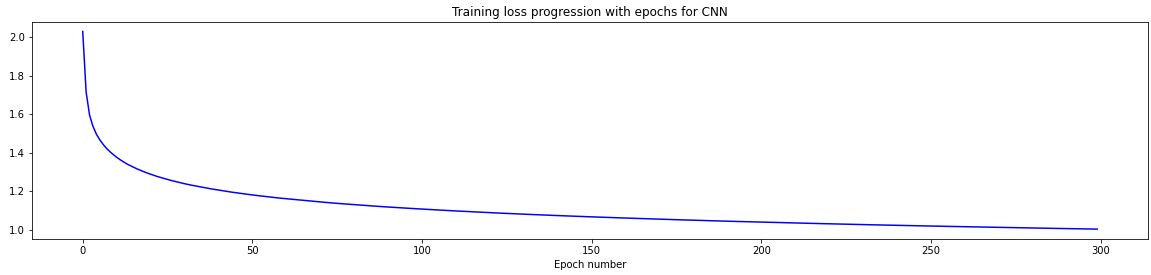
\includegraphics[width=.49\textwidth]{./images/cnnLoss.png}
	\caption{\textit{Progression of training loss of CNN in each epoch}}
	\label{fig:cnnLoss}
	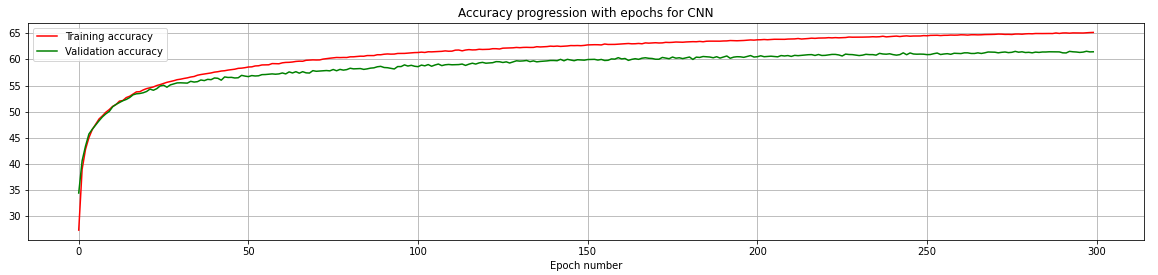
\includegraphics[width=.49\textwidth]{./images/cnnAcc.png}
	\caption{\textit{Progression of training accuracy and validation accuracy of CNN in each epoch}}
	\label{fig:cnnAcc}
\end{figure}

\section{Comparison}
Figure \ref{fig:comp} shows a summary of the performance during training of the four models tested. Note that the reason for CNN having higher training loss throughout is that it has a different loss calculating function than the rest. The testing accuracy of each model is shown in table \ref{table: tab2}.\\
We can observe that the complex models have more potential to better learn from data and make more accurate predictions. The drawback of models being more complex is that they tend to overfit the training data and fail to generalize well to unseen input. Methods like regularization, shuffling and drop-out({\small \textit{not implemented here}}) can be used to control this. The CNN has good ability to capture the spatial features of the samples instead of just pixel values and it has comparatively high accuracy thanks to this. Training on larger datasets can take long times for complex models(Currently, CIFAR-10 is considered a relatively small dataset). Methods like SGD and momentum along with efficient hardware like GPUs and TPUs can make quiet the difference in training times.\\
In conclusion, it is clear that the sophisticated models and optimization algorithms, with the help of application specific hardware can drive the machine-learning based regression and classification models to greater heights.
\begin{table}[H]
\centering
\begin{tabular}{|l|c|}
\hline
Linear model &$40.6\%$\\
Neural net w/out SGD &$43.5\%$\\
Neural net with SGD &36928\\
CNN &$60.3\%$\\
\hline
\end{tabular}
\caption{Test accuracy of each model}
\label{table: tab2}
\end{table}

\onecolumn
\begin{figure}
  \centering
	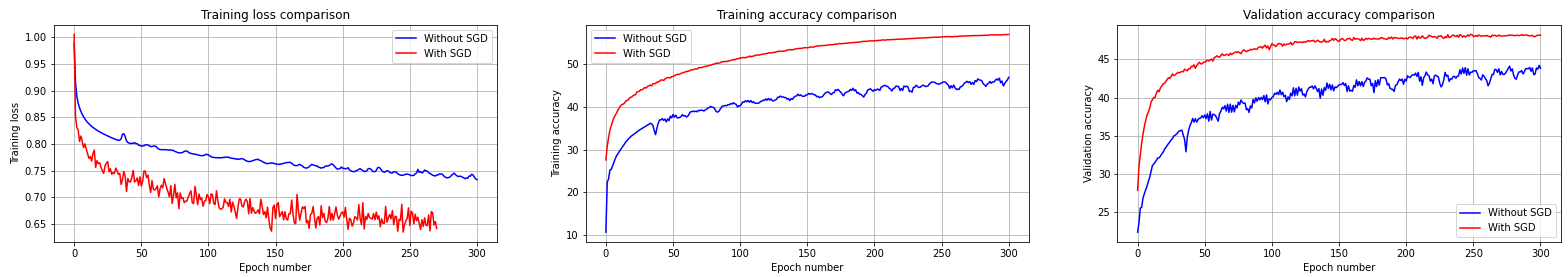
\includegraphics[width=\textwidth]{./images/nn1vs2.png}
	\caption{\textit{Comparison of training loss, training accuracy and validation accuracy of two neural network classifiers}}
	\label{fig:nn1v2}
\end{figure}
\begin{figure}
  \centering
	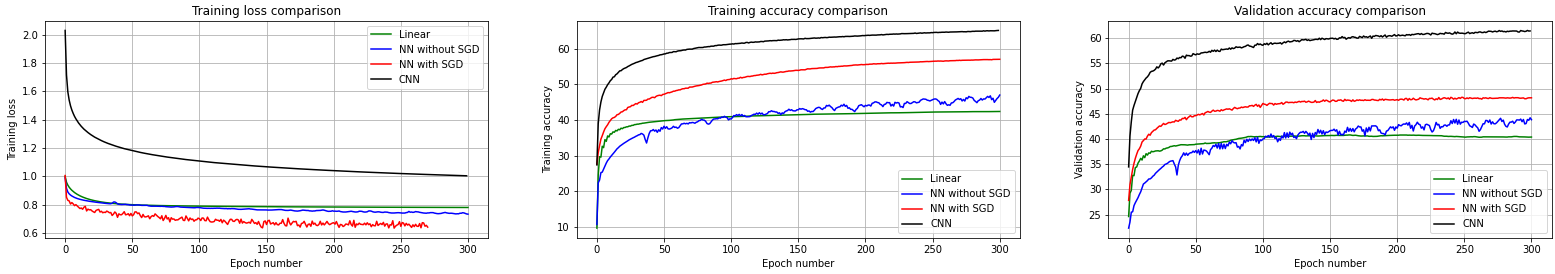
\includegraphics[width=\textwidth]{./images/compareAll.png}
	\caption{\textit{Comparison of all models}}
	\label{fig:comp}
\end{figure}
\textit{Note: The allocation of $10\%$ of training data for validation has slightly affected the training ability of, specially the three neural network based models. However, I thought of giving more importance to testing process as this models are only made to evaluate their performance and not to do any actual mission critical classification task. Therefore, I took all 10000 data as test set and got the validation split from training set. We could get higher accuracy by using 50000 data for training and taking the validation split from the test set.}

\section*{Important parts of code}
\textit{Note: Here, I have removed the 'np.' part and other data casting parts for better clarity.}
\begin{lstlisting}[frame=single,language=python,caption=Forward propagation function for linear classifier]
def forward_prop_linear(x_data, weights):
  return matmul(x_data, weights[0]) + matmul(np.ones((x_data.shape[0],1)),weights[1])
\end{lstlisting}

\begin{lstlisting}[frame=single,language=python,caption=Loss function for linear classifier]
def mean_sum_of_squared_errors_linear(y, y_hat, weights, reg=0.0):
  diff = (y_hat-y)
  return mean(sum(multiply(diff,diff),axis=1)) + reg*sum(multiply(weights[0],weights[0]))
\end{lstlisting}

\begin{lstlisting}[frame=single,language=python,caption=Backward propagation function for linear classifier]
def back_prop_linear(y_hat, y, x):
  return [np.matmul(x.T,2*(y_hat-y))/x.shape[0],np.sum(2*(y_hat-y),axis=0)/x.shape[0]]
\end{lstlisting}

\begin{lstlisting}[frame=single,language=python,caption=Gradient descent function for linear classifier]
def gradient_descent_linear(grads, weights, learning_rate=0.01, reg=0.0):
  weights[0] = weights[0]-learning_rate*grads[0]-reg*weights[0]
  weights[1] = weights[1]-learning_rate*grads[1]
  return weights
\end{lstlisting}

\begin{lstlisting}[frame=single,language=python,caption=Top-one accuracy function]
def get_accuracy(y_hat, y):
  y_hat_bin,y_class = np.argmax(y_hat,axis=1),np.argmax(y,axis=1)
  return 100*sum(y_hat_bin==y_class)/y_class.size
\end{lstlisting}

\begin{lstlisting}[frame=single,language=python,caption=Forward propagation function for neural networks]
def forward_prop_2_layer_nn(x_data, weights):
  z1 = matmul(x_data, weights[0]) + weights[1]
  a1 = sigmoid(z1)
  z2 = matmul(a1, weights[2]) + weights[3]
  return [z1,a1,z2]
\end{lstlisting}

\begin{lstlisting}[frame=single,language=python,caption=Backward propagation function for neural networks]
def back_prop_2_layer_nn(y, xs, weights):
  dz2 = 2*(xs[3]-y)/y.shape[0]
  db2 = sum(dz2,axis=0,keepdims=True)
  dW2 = matmul(xs[2].T,dz2)
  da1 = matmul(dz2,weights[2].T)
  dz1 = xs[2]*(1-xs[2])*da1
  db1 = sum(dz1,axis=0,keepdims=True)
  dW1 = matmul(xs[0].T, dz1)
  return [dW1,db1,dW2,db2]
\end{lstlisting}

Loss function and gradient descent for neural networks differ from linear model only because of having four weights instead of two and therefore, I didn't include those functions here. The neural network implementation with SGD(listing 8 below) and without SGD are similar except for the second loop which iterates over the mini-batches in SGD. The normal neural network does not need this loop as it's processing all samples at the same time.

\begin{lstlisting}[frame=single,language=python,caption=SGD implementation]
for epo in range(no_epochs+1):
  # Shuffle training data
  ind = np.arange(Ntr)
  rng.shuffle(ind)
  x_train_shuffled = x_train[ind]*100.0
  y_train_shuffled = y_train[ind]

  # Learning step down as batches
  for step in range(steps_per_epoch):
    batch = x_train_shuffled[step*batch_size: (step+1)*batch_size]
    batch_labels = y_train_shuffled[step*batch_size: (step+1)*batch_size]
    results = forward_prop_2_layer_nn(batch,weights_nn)
    y_hat = results[-1]
    loss = mean_sum_of_squared_errors_2_layer_nn(batch_labels, y_hat, weights_nn,
                                                 regularization_nn2)
    nn2_loss_history.append(loss)
    grads = back_prop_2_layer_nn(batch_labels, [batch]+results, weights_nn)
    weights = gradient_descent_2_layer_nn(grads, weights_nn, learning_rate_nn2,
                                          regularization_nn2)

  learning_rate_nn2 *= learning_rate_decay_nn2
\end{lstlisting}

\begin{lstlisting}[frame=single,language=python,caption=CNN implementation]
model = keras.Sequential([
		keras.layers.Conv2D(32, (3,3), padding='same', input_shape=(32,32,3),\
		name="C32"),
		keras.layers.MaxPooling2D(),
		keras.layers.Conv2D(64, (3,3), padding='same', name="C64_1"),
		keras.layers.MaxPooling2D(),
		keras.layers.Conv2D(64, (3,3), padding='same', name="C64_2"),
		keras.layers.MaxPooling2D(),
		keras.layers.Flatten(),
		keras.layers.Dense(64, activation='sigmoid'),
		keras.layers.Dense(10, activation='softmax')

learning_rate_cnn = 0.015
learning_rate_decay_cnn = 0.001
sgd = keras.optimizers.SGD(learning_rate_cnn, 0.5, decay=learning_rate_decay_cnn)
model.compile(optimizer=sgd, loss='categorical_crossentropy', metrics=['accuracy'])

model.fit(x_train, y_train, batch_size=50, epochs=10, validation_data=(x_val, y_val))
\end{lstlisting}

\end{document}